\chapter{Transfer Learning in One Class CF for Shopping Prediction}
\label{chp:trimf}
\section{Problem settings}
\subsection{Background}
\par{
In real-world, a person usually has different kinds of behaviour before buying one thing. For online shopping sites, Their goal is to let users buy their products, but the user-item matrix for deal is extremely sparse( less than $0.001\%$ ). So if we only use the information of deal, we can't acheive good even reasonable performance. 

In Yixun(Tencent's online shopping site), there are two main actions - click and purchase, both consists only binary data(1-action happened, 0-unknown). We know that deal matrix $X_d$ is very sparse, althrough click matrix $X_c$ is also sparse, but is much denser than $X_d$. So we developed a transfer learning algorithm(TRIMF) that leverage these data to predict a user's future purchasing. Compared with former methods which shares rating patterns or latent features only, our method shares both rating patterns and latent features throught cluster-level transform and overlapping matrix. Experiments show that my algorithm performs better then other baseline(Transfer) methods.}

\subsection{Problem definition}
  \begin{itemize}
  \item Input: [0-1 matrix:user click matrix $X_C(m_c*n_c)$, user deal matrix $X_d(m_d*n_d)$] , $m_c, m_d$ denote the number of users, $n_c, n_d$ denote the number of items. Users and items are partially shared.
  \item Output: Two prediction matrix $P_C(m_c*n_c), P_d(m_d*n_d)$, which predict users' purchasing behaviour.
  \end{itemize}



\section{TRIMF}
\subsection{Weighting scheme of TRIMF}
  \par{Former one-class CF methods ~\cite{4781121}, ~\cite{4781145} use weighted low-rank approximation to tackle the problem that all observed ratings are 1. Given a rating matrix $R = (R_{ij})_{m*n} \in \{0, 1\}^{m*n}$ with $m$ users and $n$ items and a corresponding non-negative weight matrix $W = (W_{ij})_{m*n} \in R^{m*n^+}$ , weighted low-rank approximation aims at finding a low rank matrix $X = (X_{ij})_{m*n} $minimizing the objective of a weighted Frobenius loss function as follows : $L(X) = w(R_{ij} - X_{ij})$. 

In ~\cite{4781121}, the authors consider actions that happens more than once(e.g click an item mutiple times). Negative entries are ignored, for each positive entry, its weight is propotional to its frequency, since more frequent can mean that we are more confident about the entry. In ~\cite{4781145}, positive entries are all with the same weight 1, while negative entries are considered in different ways. According to their experiments, user-oriented weighting scheme can acheive best performance. That is, for negative entries $W_{ij} \propto \sum_j{R_{ij}}$, it's idea is that if a user has more positive examples, it is more likely that she does not like the other items, that is, the missing data for this user is negative with higher probability.

In our method we adopt this weighting scheme to give missing values proper weights, i.e for positive entries we use the weighting scheme in ~\cite{4781121} and negative entries we use user-oriented weighting.}
\subsection{Transfer learning in TRIMF}

User's deal data is very sparse, e.g users will buy $n_d$ items one day while click $n_c$ items. Then $n_d \ll n_c$. So only use deal data is not sufficient. Traditional transfer learning methods use matrix factorization and share a certain part of low-rank matrix(e.g user-latent factor, rating pattern). But none of them apply multi-selective-sharing schme.

In TRIMF, rating matrix are factorized into three parts : $X = USV^T$. We want to use users' click data to learn a better cluster-level rating pattern $S$, compared with only using users' purchase data. And for overlap users and items, we want their latent vector$U,V$ to be the same, too. That it, we share their rating patterns and latent vectors. But what a user like to click is not always the item he wants to buy. So these rating pattern should be somehow related but not the same. In Yixun, there are only 2 common items in top-10 click items and top-10 purchase items (Table ~\ref{tbl:topitem}). So we can't simply apply the same pattern in prediction.

\begin{table}[h]

%\begin{Large}
\label{tbl:topitem}
\begin{center}
\begin{tabular}{| c | c |}
\hline
Top click items & Top purchase items \\
\hline
Iphone 5s & Tissue\\
Xiaomi 3 & Laundry soap powder\\
Thinkpad & Xiaomi 3\\
CPU & Snacks\\
Hard disk & Battery\\
Router & Iphone 5s\\
Earphone & Mouse\\
\hline
\end{tabular}
\caption{Top 10 click items and top 10 purchase items in Yixun}
\end{center}
%\end{Large}
\end{table}

\par{However, after careful observation we found that there are some items which belongs to the same category with higher conversion rate(user tends to buy after clicking), but some categories not. And there are some users who like window-shopping while others will buy it right after clicking. These are all cluster-level features, we design a mapping function to let the learnt $S$ suit data better.}

\subsection{Object function}
\par{We use a weighted non-negative matrix tri-factorization method to deal with the problem as illustrated below. 
\begin{figure}

%\begin{Large}

\begin{center}
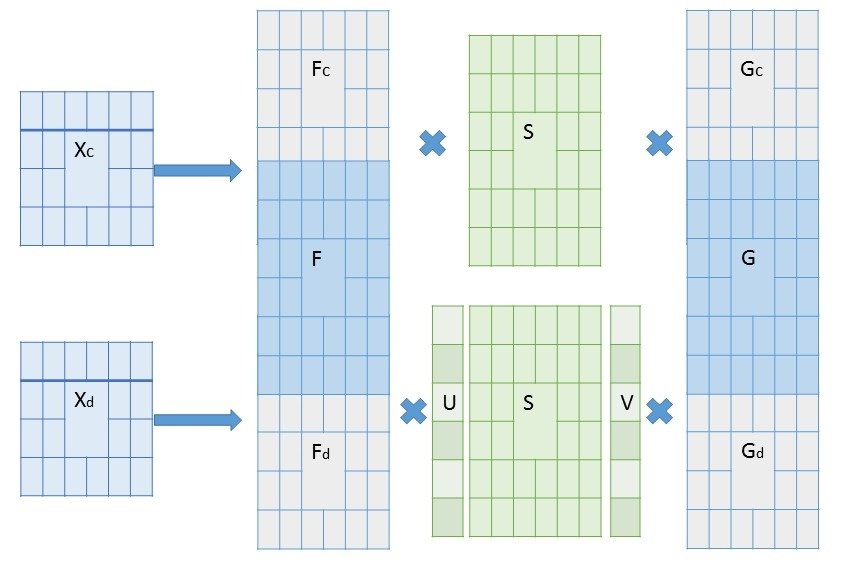
\includegraphics[width=400px]{fig/trimf.jpg} 
\caption{Graphical model of TRIMF}
\label{fig:trimf}
\end{center}
\end{figure}}
 
  \par{Objective Function:$$min_{F,G,S,U,V} W_c\odot ||X_c - (F;F_c)S(G;G_c)'||_2 + W_d\odot ||X_d - (F;F_d)(USV)(G;G_d)'||_2 $$}

  \par{
    \begin{itemize}
    \item $W_c,W_d$ is the weight for $X_C, X_d$, every observed entry has weight $1 + log(frequency)$. while others have weight $W_{ij} = \sum_jI({R_{ij}})$.
    \item $F, G$ is the soft clustering result matrix for overlapped users(items), they are forced to have the same cluster distributions. Others are unique users(items).
    \item $U,V$ are two diagonal matrix, $U_{ii}$ scales every $S_{i*}$ to $U_{ii}S_{i*}$, it models the users' tranform from click to deal. While $V_{jj}$ scales every $S_{*j}$ to $S_{*j}V_{jj}$, it models the items' tranform from click to deal.
    \item When predicting, we use $(F;F_d)(USV)(G;G_d)$ to predict users who have deal data. And since we got two mapping matrix $U,V$, we apply $U,V$ back to click matrix to predict users who have click data, i.e we use $(F;F_c)(USV)(G;G_c)$ to predict.
    \end{itemize}
}



\begin{section}
  {Solution to TRIMF \& Algorithm}
\par{Follow the update rules in ~\cite{Zhuang:2011:EAW:1952191.1952195}, we use an alternately iterative algorithm to solve the objective function.}

Firstly, we declare some denotions:
\begin{itemize}
	\item $Ic,Icc,Icd,Id$ : $(Ic,Icc)*(F;F_c) = I*(F;F_c)$ and $(Icd,Id)*(F;F_d) = I*(F;F_d)$
	\item $sg$ : $S*G'*G*S'$
	\item $F_1, F_2$ : $[F;F_c]$, $[F;F_d]$
\end{itemize}
\par{In each round of iteration these matrixes are updated as :
$$F \leftarrow F .* \sqrt{\frac{Icc'*(W_c.*X_c)*G*S' + Icd'*(W_d.*X_d)*G*S'}{(Icc'*Icc*F + Icc'*Ic*F_c + Icd'*(Icd*F + Id*F_d))*sg)}}$$
$$F_c \leftarrow F_c .* \sqrt{\frac{Ic'*(W_c.*X_c)*G*S'}{Ic'*(Icc*F + Ic*F_c)*sg}}$$
$$F_d \leftarrow F_d .* \sqrt{\frac{Id'*(W_d.*X_d)*G*S'}{Id'*(Icd*F + Id*F_d)*sg }}$$
$$G \leftarrow G .* \sqrt{\frac{W_c.*X_c*F_1*S + (W_d.*X_d)'*F_2*S}{(G*(S'*F_1'*F_1*S + S'*F_2'*F_2*S)}}$$
$$U \leftarrow U .* \sqrt{\frac{F_2'*(W_d.*X_d)*G*V'*S'}{F_2'*F_2*U*S*V*G'*G*V'*S'}}$$
$$V \leftarrow V .* \sqrt{\frac{S'*F_2'*(W_d.*X_d)*G}{S'*F_2'*F_2*S*V*G'*G}} $$



}

\par{The user-item matrix is typically very sparse with $z \ll nm$ non-zero entries while $k$ is typically
also much smaller than n, m. By using sparse matrix multiplications and avoiding dense intermediate matrices, the updates can be very efficiently
and easily implemented. In particular, updating F, S, G each takes $O(k^2 (m + n) + kz)$ , and the algorithm usually reach convergence in less than 200 iterations.}

\begin{algorithm}[tb]
\caption{Algorithm for TRIMF.}
\begin{algorithmic}

\STATE {\bfseries Input:} $\X_{c}$, $\X_{d}$\\
$\X_{c} \in \mathbb{R}^{m_c\times n_c}$: the purchase data \\
$\X_{d} \in \mathbb{R}^{m_d\times n_d}$: the click data\\

\STATE {\bfseries Initialize:} Initialize $W_c, W_d$ : $(1+log(freq))$ for observed, $\sum_jI({R_{ij}})$ for unseen, $F,G,S,U,V$ : $random$, Set overlap numbers for users and items

\FOR{ $i$ = 1 to $T$}

\STATE update $F$

\STATE update $F_c$, $F_d$

\STATE  update $G$

\STATE  update $S$

\STATE  update $U, V$


\ENDFOR

\STATE {\bfseries Output:} $F,G,S,U,V$

\end{algorithmic}
\label{algorithm:TRIMF}
\end{algorithm}

\end{section}
\begin{section}{Experiment}
  \begin{subsection}{Datasets}

We select real data from an online shopping site: yixun.com \footnote{http://www.yixun.com}. We collect data for 6 months, the entire dataset consists 5,324,231 users and 643,123 items. The sparsity in click matrix is $0.06\%$, in purchase matrix is $0.0003\%$.

To check the effectiveness of TRIMF in short time and long time, we construct two smaller datasets.

\begin{itemize}

\item \textbf{Yixun short term data}: we select data from two weeks, 20130801-20130814. we sample a fraction of user by random, and remove those whose action frequency is too low(e.g only one click during this period). In the click matrix we have 16240 users and 1932 items. In the purchase matrix we have 2520 users and 1791 items. There are 2029 overlapped users and 1642 overlapped items. We train our model using data from first week and data from second week is used for testing.
\item \textbf{Yixun long term data}: we select 1012 active users through 6 months. In their long term actions, there are 6021 items which have been clicked and 1973 items boughted. We select the five latest purchasing items per user as test data, others as training data. There are 1503 overlapped items.

\end{itemize}
\end{subsection}

\begin{subsection}{Metrics}
We use $prec@5$ and $prec@10$ as our evaluation meatures. $prec@n$ is the precision of top-n results. Our main goal is to optimize for conversion rate(future purchase matrix), so the test is mainly done in the purchase matrix. However, since TRIMF can also optimize for source domain(click matrix), some test in click matrix is also conducted.

  
\end{subsection}

\begin{subsection}{Baseline methods}  

We divide baseline methods into non-transfer methods and transfer methods. All baseline methods are shown in Table \ref{baseline}.
\begin{table}

\begin{center}
  \begin{tabular}{|c|c|}
    \hline
    non-transfer methods & transfer methods\\
    \hline
    Most Popular, SVD, NMF, PMF, BPRMF, WRMF&CMF, TCF, TRIMF\\
\hline
  \end{tabular}
\end{center}
\caption{Baseline methods.}
\label{baseline}


\end{table}
\subsubsection{non-transfer methods}
\par{
  For all non-transfer methods, we use 3 combinations of matrix as our training matrix:{deal, click, deal+click}, and report their best performace. We choose parameters by cross validation.
  \begin{itemize}
    \item Most Popular: Most popular selects top-n items in global, and provide same recommendation results for each user.
    \item SVD ~\cite{paterek07}: Singular Value Decomposition(SVD) is a typical method used in recommender system, here PureSVD from Matlab is used.
      \begin{itemize}
      \item rank = \{5,10,20,30,40,50\}
      \end{itemize}
    \item NMF ~\cite{/computer/yehuda09matrix}: Non-negative Matrix Factorization(NMF) is also a typical method used in recommender system, here NMF from Matlab is used.
      \begin{itemize}
      \item rank = \{10,20,40,60,100\}
      \end{itemize}
    \item PMF ~\cite{/nips/SalMnih08}:Probabilistic Matrix Factorization(PMF) is a recently proposed method for missing value prediction. Previous work showed that this method worked well on the large, sparse and imbalanced data set.
      \begin{itemize}
      \item rank = \{10,20,30,40,50\}
      \end{itemize}
    \item BPRMF ~\cite{Rendle:2009:BBP:1795114.1795167}: BPR is a generic optimization criterion for personalized ranking that is the maximum posterior estimator derived from a Bayesian analysis of the problem. Unlike traditional methods whose object function is point-wise, BPR is a pair-wise object function. BPRMF implements BPR using matrix factorization.
      \begin{itemize}
      \item We initialized BPR with most popular results.
      \item We set $iteration = \#n * 100$, ($\#n$ in the number of observations)
      \end{itemize}
    \item WRMF ~\cite{4781145}: One-class collaborative filtering(WRMF) is a weighted low rank approximation method optimized for implicit dataset. 
      \begin{itemize}
      \item rank = \{5,10,15,20,25\}
    \end{itemize}
\end{itemize}
\subsubsection{transfer methods}
\begin{itemize}
    \item CMF ~\cite{/kdd/SinghG08}:Collective Matrix Factorization is proposed for jointly factorizing two matrices. Being adopted as a transfer
learning technique in several recent works, CMF has been proven to be an effective cross-domain recommendation approach. For each training and testing pairs, we make two matrix the same dimension(in order to share a latent factor) by padding rows \& columns.
      \begin{itemize}
      \item Shared latent space dimension = \{5,10,15,20,25\}
      \end{itemize}
    \item TCF ~\cite{/ijcai/PanLXY11}: TCF is a transfer learning method to predict missing ratings via heterogeneous feedbacks. It's originally designed for rating prediction, so we set the deal matrix with random sampled zeros as the rating matrix, click matrix as the implicit feed back matrix. Zero rows and colomns are also padded to make the two matrix in same dimension.
\item TRIMF: our method.
  \begin{itemize}
  \item We set latent factor = 30, iteration = 200.
  \end{itemize}
    \end{itemize}
  
}
\end{subsection}
\end{section}
\subsection{Results}
  \begin{subsubsection}{Yixun short term data}
\par{Since the user overlap of deal and click matrix are small, so we perform two test, one on deal matrix $X_d$ and one on click matrix $X_c$.}
\par{Results are showed in Table \ref{shortdeal} and Table \ref{shortclick}.}
\begin{table}


\begin{center}
  \begin{tabular}{|c|c|c|}
    \hline
    Method&Prec@5&Prec@10\\
    \hline
    Most Popular&0.0323&0.0289\\
    \hline
    SVD&0.0438&0.0367\\
    \hline
    NMF&0.0403&0.0324\\
    \hline
    PMF&0.0435&0.0372\\
    \hline
    BPRMF&0.0444&0.0364\\
    \hline
    WRMF&0.049&0.0403\\
    \hline
    CMF&0.0436&0.0350\\
    \hline
    TCF&0.0453&0.0369\\
    \hline
    TRIMF&\textbf{\color{red}0.0525}&\textbf{\color{red}0.0410}\\
    \hline
  \end{tabular}
\end{center}
\caption{Performance of TRIMF and other baseline methods on short-term users who have deal data.}
\label{shortdeal}

\end{table}

\begin{table}

  \centering


  \begin{tabular}{|c|c|c|}
    \hline
    Method&Prec@5&Prec@10\\
    \hline
    Most Popular&0.0090&0.0085\\
    \hline
    SVD&0.0123&0.00113\\
    \hline
    NMF&0.0091&0.0089\\
    \hline
    PMF&0.0121&0.0112\\
    \hline
    BPRMF&0.0142&0.0130\\
    \hline
    WRMF&0.0174&0.0144\\
    \hline
    CMF&0.0176&0.0139\\
    \hline
    TCF&0.0158&0.0127\\
    \hline
    TRIMF&\textbf{\color{red}0.0189}&\textbf{\color{red}0.0153}\\
    \hline
    TRIMF(without remap)&0.0175&0.0146\\
    \hline
  \end{tabular}
\caption{Performance of TRIMF and other baseline methods on short-term users who have deal data.}
  \label{shortclick}
  
\end{table}
\end{subsubsection}


\begin{subsubsection}
  {Yixun long term data}
\par{Since the user are manually selected, we only test $X_d$. The result is showed in Table \ref{longterm}.}

\begin{table}
  \centering
  \begin{tabular}{|c|c|c|}
    \hline
    Method&Prec@5&Prec@10\\
    \hline
    Most Popular&0.00508&0.00405\\
    \hline
    SVD&0.00453&0.00413\\
    \hline
    NMF&0.00401&0.00389\\
    \hline
    PMF&0.00421&0.00312\\
    \hline
    BPRMF&0.00542&0.00430\\
    \hline
    WRMF&0.00485&0.00345\\
    \hline
    CMF&0.00512&0.00432\\
    \hline
    TCF&0.00534&0.00502\\
    \hline
    TRIMF&\textbf{\color{red}0.00720}&\textbf{\color{red}0.00606}\\
    \hline
  \end{tabular}
  \caption{Performance of TRIMF and other baseline methods on long-term users.}
\label{longterm}
\end{table}
\end{subsubsection}



\begin{section}{Performance comparison \& analysis}
First, we observed that TRIMF out-perform all other baseline non-transfer methods in three tests. In short-term deal test, we can see traditional CF method which aims at rating prediction (e.g SVD, NMF) can't achieve compatible performance than others. Because these methods is designed for matrix with multiple values, not for our binary matrix. while CF method designed for binary matrix(BPRMF, WRMF) can acheive significantly greater result. In long-term test the difference is not so significant, because the data here is less sparse than short-term data, every method has enough data to train a good model.

Second, TRIMF also out-perform other transfer methods. Since CMF, TCF are also designed for rating prediction problems. The information in our training set is limited, so both methods can't transfer enough knowledge from their framework. TRIMF is designed for one-class transfer learning, TRIMF combines one-class and transfer methods, so it inherits advantages from both side.

  \subsubsection{The effects of $UV$}
In our assumption, $UV$ are two mapping matrix that describe the difference in user-cluster and item-category. To see whether $UV$ really reflects the phenomenon, we manually check entries in $UV$ with high and low values.

  We found that high value in $V$ reflects item clusters that people tends to buy after clicking, e.g toothbrush, snacks. While low value of $V$ more reflects that items are popular but people may not buy it immediately, e.g cell phones, laptops. High value in $U$ reflects user-cluster who tends to buy after clicking, while users belong to low value user-clusters are all window-shopping fans.

  In Table \ref{shortclick}, we can see if we want to predict future purchasing items on users who have click data, we can map $UV$ back. Thus the learned cluster-pattern $S$ is transformed from click pattern to purchase pattern.

  \subsubsection{The effects of sharing}
    To see that sharing $F,G$ really works, we select another 6000 users to test, we tried 'not share','share' and 'random share', the $prec@n$ here are not comparable with the first experiment(Table \ref{shortdeal}). Results show that we must share latent factor carefully, random share may do harm to performance. But sharing latent factor for overlapped users/items can achieve a significantly greater result.

    \par{
\begin{table}
\begin{center}
  \begin{tabular}{|c|c|c|}
    \hline
    Method&Prec@5&Prec@10\\
    \hline
    shareFG&\textbf{\color{red}0.0436}&\textbf{\color{red}0.0350}\\
    \hline
    not share&0.0335&0.0306\\
    \hline
    random share&0.0344&0.0299\\
    \hline
  \end{tabular}
\end{center}
\caption{The effect of sharing}
\label{sharing}
\end{table}
}
\end{section}

